\documentclass[journal,compsoc]{IEEEtran}

% ── Packages ──────────────────────────────────────────────────────────────
\usepackage[T1]{fontenc}
\usepackage[utf8]{inputenc}
\usepackage{amsmath,amssymb,amsthm}
\usepackage{mathtools}
\usepackage{booktabs}
\usepackage{tabularx}
\usepackage{multirow}
\usepackage{graphicx}
\usepackage{xcolor}
\usepackage{hyperref}
\usepackage{url}
\usepackage{cite}
\usepackage{microtype}
\usepackage{ragged2e}
\usepackage{balance}
\usepackage[ruled,vlined,linesnumbered]{algorithm2e}
\usepackage{tcolorbox}
\usepackage{pgfplots}
\usepackage{tikz}
\usetikzlibrary{arrows.meta,positioning,fit,backgrounds,calc,patterns}
\pgfplotsset{compat=1.18}

% ── Custom commands ─────────────────────────────────────────────────────
\newcommand{\HEPI}{\textsc{HEPI}}          % Novel metric: HE Privacy Index (text-safe; use \mathrm{HEPI} inline in math)
\newcommand{\framework}{\textsc{HE-MedInfer}}
\newcommand{\Enc}{\mathcal{E}}
\newcommand{\Dat}{\mathcal{D}}
\newcommand{\Mod}{\mathcal{M}}
\newcommand{\checkyes}{\checkmark}
\newcommand{\checkno}{$\times$}

% ---- Document ----------------------------------------------------------------
\begin{document}

\title{Homomorphic Encryption-Enabled Secure Machine Learning Inference for
       Privacy-Compliant Healthcare Diagnostics Without Data Decryption}

\author{Allan~Douglas~Costa,~\IEEEmembership{Member,~IEEE}%
\thanks{A.~D.~Costa is with the Federal Rural University of the Amazon (UFRA),
Institute of Computing and Information and Communication Technology (ICIBE),
Bel\'{e}m, Par\'{a}, Brazil.
E-mail: allan.costa@ufra.edu.br | ORCID: 0000-0002-7068-8889}%
\thanks{Reproducibility: the \framework{} reference implementation, the
synthetic data generator, and all scripts required to regenerate every figure
and table in this paper are released under the MIT license at
\url{https://github.com/sec365/he-medinfer}.}}

\markboth{IEEE Transactions on Information Forensics and Security}{}

\maketitle

% =============================================================================
\begin{abstract}
% [Topic]
The proliferation of machine learning in clinical decision support systems has
created an urgent demand for inference pipelines that operate directly on
sensitive patient data without ever exposing it in plaintext.
% [Motivation]
Regulatory frameworks such as HIPAA and GDPR impose strict constraints on
healthcare data processing, yet existing privacy-preserving inference approaches
incur prohibitive latency or require partial decryption at intermediate stages,
creating compliance gaps that undermine patient trust.
% [Contribution]
We propose \framework{}, a three-tier homomorphic encryption (HE) framework
that enables end-to-end encrypted machine learning inference for healthcare
diagnostics, requiring no data decryption at any point in the inference
pipeline.
% [Detail]
\framework{} integrates CKKS-based approximate arithmetic with a novel
polynomial approximation strategy for non-linear activation functions, and
introduces the \emph{HE Privacy Index} (\HEPI{}), a composite metric that
jointly quantifies ciphertext security, computational overhead, and inference
accuracy degradation under encrypted computation.
% [Evidence]
We evaluate \framework{} on \emph{synthetic clinical data generated to match
published MIMIC-III summary statistics} for the in-hospital mortality
prediction task, using a three-agent architecture (Encryption Agent, Inference
Agent, Audit Agent). Under full HE, \framework{} attains an AUROC of 0.856
(accuracy 91.7\%) against a plaintext upper bound of 0.871 (93.8\%), yielding
a mean \HEPI{} of 0.886.
% [Weaker result]
Inference latency remains 14.3$\times$ higher than plaintext baselines, and
because our evaluation is simulation-based rather than executed on the
restricted-access MIMIC-III records themselves, the reported accuracies
establish internal consistency of the pipeline rather than externally
validated clinical performance.
% [Narrow impact]
Healthcare organizations can deploy \framework{} to achieve HIPAA/GDPR
compliance without sacrificing diagnostic utility or requiring trust in
cloud infrastructure.
% [Broad impact]
This work advances the broader agenda of privacy-by-design AI, enabling
responsible deployment of clinical AI in jurisdictions with strict data
sovereignty requirements.
\end{abstract}

\begin{IEEEkeywords}
Homomorphic encryption, privacy-preserving machine learning, secure inference,
healthcare AI, CKKS, HIPAA compliance, GDPR, federated diagnostics,
HE Privacy Index.
\end{IEEEkeywords}

% =============================================================================
\section{Introduction}
\label{sec:intro}

Artificial intelligence is rapidly transforming clinical medicine, enabling
diagnostic systems that match or surpass specialist-level performance in tasks
ranging from radiological image interpretation to early sepsis detection
\cite{rajpurkar2022ai,topol2023highperformance,esteva2019guide,miotto2018deep,
chowdhury2023survey,natarajan2023clinicalml}.
However, the deployment of machine learning inference in production healthcare
environments requires that patient data traverse untrusted computational
infrastructure, including cloud platforms, third-party APIs, and shared
hospital networks, creating substantial privacy risks
\cite{price2019privacy,chen2024ehr}. Multi-institutional deployments of
diagnostic AI further compound this risk, as model training and inference
pipelines routinely aggregate imaging and tabular records across
administratively independent hospitals \cite{kaissis2021endtoend}.

Regulatory frameworks governing health data impose strict constraints on this
pipeline. The U.S. Health Insurance Portability and Accountability Act (HIPAA)
mandates that protected health information (PHI) be secured against unauthorized
disclosure at rest and in transit \cite{edemekong2023hipaa}, while the European
General Data Protection Regulation (GDPR) requires a legal basis for any
processing of special-category data, which includes health records
\cite{voigt2017gdpr}. Yet most deployed clinical AI systems require data to be
decrypted prior to inference, creating a compliance gap: the moment plaintext
data touches an inference server, the healthcare provider bears the full
regulatory burden of securing that computation environment.

Homomorphic encryption (HE) offers a principled solution: it allows arbitrary
computations to be performed directly on ciphertexts, producing an encrypted
result that, when decrypted by the authorized key holder, matches the output
of the same computation on the original plaintext \cite{gentry2009fully}.
Applied to machine learning inference, HE eliminates the requirement for data
decryption at the inference server, fundamentally shifting the trust model of
clinical AI deployment.

Despite this promise, HE-based inference in healthcare remains underexplored.
Prior works, such as CryptoNets \cite{gilad2016cryptonets} and HEMET
\cite{lou2021hemet}, demonstrate the feasibility of encrypted neural network
inference on benchmark datasets (MNIST, CIFAR-10) but do not address the
specific challenges of clinical data: high-dimensional tabular features,
mixed data types, and the accuracy sensitivity of diagnostic applications.
The closest work to ours, Lee et al.~\cite{lee2022privacypreserving},
demonstrates privacy-preserving deep learning via CKKS homomorphic encryption
but does not address compliance auditing, multi-party clinical scenarios, or
the joint optimization of security strength and accuracy degradation, which
motivates our proposed \framework{} framework.

\subsection*{Contributions}

This paper makes the following contributions:

\begin{enumerate}
  \item We propose \framework{}, a three-tier encrypted inference framework
    for healthcare diagnostics that operates end-to-end under CKKS homomorphic
    encryption, requiring no plaintext exposure at any inference stage.

  \item We introduce the \emph{HE Privacy Index} (\HEPI{}), a novel composite
    metric that jointly quantifies ciphertext security strength, computational
    overhead relative to plaintext inference, and accuracy degradation under
    encrypted computation, enabling principled trade-off analysis for
    HE-based clinical AI deployment.

  \item We design and evaluate a three-agent architecture (Encryption Agent,
    Inference Agent, Audit Agent) with independent performance metrics per
    agent, demonstrating that the framework's overhead is localized and
    predictable.

  \item We provide a formal compliance mapping of \framework{} against HIPAA
    Security Rule, GDPR Article 25 (data protection by design), and NIST
    SP 800-111, demonstrating that the framework satisfies all principal
    regulatory controls for encrypted health data processing.

  \item We evaluate \framework{} on a fully specified synthetic clinical
    cohort calibrated to published MIMIC-III~\cite{johnson2016mimic} summary
    statistics for in-hospital mortality prediction, reporting AUROC,
    calibration error, and accuracy against a majority-class reference,
    together with 95\% confidence intervals, a Mann-Whitney $U$
    test~\cite{mann1947test}, ablation studies, and comparison against three
    baselines. The generator and evaluation harness are released so that the
    entire result set is reproducible without restricted-access credentials.
\end{enumerate}

\subsection*{Scope of Evidence}

We state the evidentiary scope of this work explicitly, because it bounds every
empirical claim that follows. All reported accuracies, latencies, and \HEPI{}
scores are obtained on \emph{synthetic} records drawn from a generative model
whose marginal distributions, missingness pattern, and outcome prevalence are
fitted to published MIMIC-III summary statistics
(Section~\ref{sec:datagen}); we did not execute the pipeline on the
restricted-access MIMIC-III records themselves. Consequently, the cryptographic
and systems results (ciphertext sizes, homomorphic circuit depth, latency,
throughput, audit-log consistency) are exact, since they depend only on the
CKKS parameters and the model architecture rather than on the data values,
whereas the diagnostic-utility results (AUROC, calibration, accuracy) are
\emph{internally} valid and should be read as establishing the consistency and
reproducibility of the pipeline, not as externally validated clinical
performance. Validation on real MIMIC-III records under an executed Data Use
Agreement is the immediate next step and is stated as such in
Section~\ref{sec:discussion}.

The remainder of this paper is organized as follows. Section~\ref{sec:related}
reviews related work and positions \framework{} against the state of the art.
Section~\ref{sec:threat} formalizes the threat model and defines \HEPI{}.
Section~\ref{sec:framework} details the \framework{} architecture and
algorithms. Section~\ref{sec:security} presents the security and compliance
analysis. Section~\ref{sec:eval} reports experimental results.
Section~\ref{sec:discussion} discusses findings, limitations, and threats to
validity. Section~\ref{sec:conclusion} concludes.

% =============================================================================
\section{Background and Related Work}
\label{sec:related}

\subsection{Homomorphic Encryption}

Gentry's seminal construction \cite{gentry2009fully} established the
theoretical foundation for fully homomorphic encryption (FHE), enabling
arbitrary computation over ciphertexts. Practical HE schemes relevant to
machine learning include the CKKS scheme \cite{cheon2017ckks}, which supports
approximate arithmetic over fixed-point numbers and is well-suited to the
floating-point operations central to neural network inference. The BFV scheme
\cite{fan2012bfv} targets exact integer arithmetic and is appropriate for
models with discretized parameters, and CHIMERA \cite{boura2018chimera}
demonstrates that CKKS, BFV, and boolean HE schemes can be composed within a
single circuit via scheme switching, at the cost of additional bootstrapping
overhead that is difficult to amortize in latency-sensitive clinical pipelines.
Wood et al.~\cite{wood2020homomorphic}
survey applications of HE to medicine and bioinformatics, concluding that
CKKS-based approaches offer the most practical trade-off for healthcare ML
inference given the approximate nature of clinical numerical data. However,
their survey does not address multi-agent compliance architectures or
provide a unified metric for evaluating the security-accuracy-performance
trade-off. Open-source HE toolchains such as the SEAL-based CryptoML library
\cite{chen2022cryptoml} lower the engineering barrier for CKKS deployment but
leave parameter selection and accuracy calibration to the application
developer, a gap \framework{} addresses through its Encryption Agent.

\subsection{Privacy-Preserving Machine Learning}

Mohassel and Zhang's SecureML \cite{mohassel2017secureml} introduces
a mixed-protocol framework combining secret sharing and HE for privacy-preserving
logistic regression and neural network training. While SecureML achieves strong
security guarantees, it requires a two-server model with a non-colluding
assumption that is difficult to satisfy in healthcare cloud deployments.
CryptoNets \cite{gilad2016cryptonets} pioneered HE-based neural network
inference, achieving 98.95\% accuracy on MNIST under encryption, but its
design relies on polynomial approximations of activations that incur significant
accuracy loss on complex clinical feature distributions. Boemer et
al.~\cite{boemer2020mp2ml} propose MP2ML, a mixed-protocol framework combining
HE with garbled circuits for non-polynomial activations, reducing accuracy
loss relative to pure polynomial approximation, but at the cost of an
interactive multi-round protocol that is incompatible with our non-interactive,
single-round-trip inference requirement. PEGASUS
\cite{lu2024private} bridges polynomial and non-polynomial HE evaluation via
efficient ciphertext-to-ciphertext bootstrapping, improving activation
accuracy, yet its evaluation targets generic benchmark models rather than
clinical tabular data and does not report a compliance-oriented metric.
Generic secure-computation frameworks such as PySyft
\cite{ryffel2018generic} and FALCON \cite{wagh2020falcon} extend
privacy-preserving inference to honest-majority multi-party settings, but
both assume the presence of multiple independent computing parties, an
assumption that does not hold in the common single-cloud-provider deployment
model of most healthcare institutions.

\subsection{Federated Learning for Healthcare}

Federated learning (FL) reduces data exposure by training models locally and
aggregating gradients, but gradients remain susceptible to reconstruction
attacks \cite{zhu2023securehealth}. Zhang et al.~\cite{zhang2023survey}
survey FL applications in healthcare, identifying communication overhead and
inference-time privacy as open challenges beyond the training phase itself.
Combining FL with HE addresses part of this
gap: POSEIDON \cite{sav2021poseidon} demonstrates privacy-preserving federated
neural network learning across clinical institutions via lattice-based HE,
while Froelicher et al.~\cite{froelicher2021scalable} show scalable distributed
learning under threshold HE, and Ma et al.~\cite{ma2022federated} propose a
multi-key HE scheme that avoids a single trusted key holder in federated
aggregation. Xu et al.~\cite{xu2019hybridalpha} combine functional encryption
with differential privacy in HybridAlpha, and Zhou et
al.~\cite{zhou2023privacypreserving2} revisit functional-encryption-based FL
to reduce per-round key management cost. VerifyNet \cite{xu2024heprivacy}
adds verifiability guarantees to federated aggregation but assumes an
honest majority of participating institutions. None of these works addresses
inference-time encryption (as opposed to training-time) in a
compliance-aware, single-institution deployment framework, which is the
scenario \framework{} targets.

\subsection{Homomorphic Encryption in Clinical Applications}

A smaller body of work applies HE directly to clinical prediction tasks.
Kim et al.~\cite{kim2018logreg} implement HE-based logistic regression for
clinical risk scoring, reporting practical runtimes for linear models but not
extending their approach to deep architectures. Vizitiu et
al.~\cite{vizitiu2021applying} apply HE to deep neural networks over medical
imaging features, observing accuracy degradation comparable to the gap we
report for tabular data. Kocabas and Soyata~\cite{kocabas2022privacypreserving}
outline an HE pipeline for medical image analysis but stop at a feasibility
study without a deployable audit mechanism. MedCo
\cite{raisaro2018medco} enables privacy-preserving exploration of distributed
clinical and genomic data under threshold HE, targeting cohort-level queries
rather than per-patient diagnostic inference. Batchelor et
al.~\cite{batchelor2024heml} present an efficient homomorphic evaluation of
$k$-NN classifiers, illustrating that non-parametric models remain costly
under HE relative to the parametric MLP architecture adopted in \framework{}.
Collectively, these works confirm the feasibility of HE-based clinical
inference but leave open the joint treatment of regulatory compliance,
multi-agent auditability, and a principled trade-off metric, which is the
gap that motivates the present work.

\subsection{Baseline: Lee et al.\ (2022)}

Lee et al.~\cite{lee2022privacypreserving} present a CKKS-based privacy-
preserving deep learning framework evaluated on MNIST, CIFAR-10, and a small
medical imaging dataset, reporting less than 1\% accuracy loss relative to
plaintext inference for CNN architectures. Their framework performs well on
homogeneous image data but does not address (i)~heterogeneous clinical tabular
features, (ii)~multi-party inference with separated key management, (iii)~formal
compliance mapping to HIPAA/GDPR, or (iv)~a principled metric for quantifying
the joint security-accuracy-overhead trade-off. These gaps directly motivate
\framework{} and our proposed \HEPI{} metric.

\subsection{Comparative Analysis}

Table~\ref{tab:related} positions \framework{} against representative works
across seven evaluation criteria.

\begin{table*}[t]
\caption{Comparison of Related Privacy-Preserving Inference Approaches}
\label{tab:related}
\setlength{\tabcolsep}{4pt}
\begin{tabularx}{\textwidth}{@{}l X X X X X X c@{}}
\toprule
\textbf{Work} & \textbf{Scheme} & \textbf{Clinical Data} & \textbf{No Partial Decrypt} & \textbf{3-Agent} & \textbf{Compliance Map} & \textbf{Novel Metric} & \textbf{Year} \\
\midrule
Lee et al.~\cite{lee2022privacypreserving} (baseline) & CKKS & \checkno & \checkyes & \checkno & \checkno & \checkno & 2022 \\
CryptoNets~\cite{gilad2016cryptonets}      & YASHE~\cite{bos2013yashe} & \checkno & \checkyes & \checkno & \checkno & \checkno & 2016 \\
POSEIDON~\cite{sav2021poseidon}            & LHE  & \checkno & \checkyes & \checkno & \checkno & \checkno & 2021 \\
SecureML~\cite{mohassel2017secureml}       & HE+SS & \checkno & \checkno  & \checkno & \checkno & \checkno & 2017 \\
Wood et al.~\cite{wood2020homomorphic}     & Survey & \checkyes & N/A      & \checkno & \checkno & \checkno & 2020 \\
Ran et al.~\cite{ran2023inferring}         & CKKS & \checkno & \checkyes & \checkno & \checkno & \checkno & 2023 \\
Ali et al.~\cite{ali2023secure}            & BFV  & \checkyes & \checkno  & \checkno & \checkno & \checkno & 2023 \\
Kim et al.~\cite{kim2018logreg}              & CKKS & \checkyes & \checkyes & \checkno & \checkno & \checkno & 2018 \\
Vizitiu et al.~\cite{vizitiu2021applying}  & MORE & \checkyes & \checkyes & \checkno & \checkno & \checkno & 2020 \\
MedCo~\cite{raisaro2018medco}              & Threshold & \checkyes & \checkyes & \checkno & \checkno & \checkno & 2018 \\
\midrule
\textbf{\framework{} (ours)}               & \textbf{CKKS} & \textbf{\checkyes} & \textbf{\checkyes} & \textbf{\checkyes} & \textbf{\checkyes} & \textbf{\HEPI{}} & \textbf{2026} \\
\bottomrule
\end{tabularx}
\end{table*}

% =============================================================================
\section{Threat Model and Problem Formulation}
\label{sec:threat}

\subsection{System Entities}

We consider three principals: (i)~\emph{Data Owner} (DO), a healthcare
institution holding patient records; (ii)~\emph{Inference Server} (IS), a
cloud or third-party platform performing ML inference; and
(iii)~\emph{Key Authority} (KA), a trusted entity managing CKKS key generation
and distribution.

\subsection{Threat Model}

We adopt a \emph{honest-but-curious} adversary model for the Inference Server:
the IS executes the inference protocol correctly but may attempt to learn
sensitive information from the data and intermediate computations it observes.
We additionally consider an \emph{external eavesdropper} who may intercept
ciphertexts in transit. We do not consider malicious DO or KA, and we assume
secure channels between all parties via TLS 1.3 with mutual authentication.

\subsubsection*{On the adequacy of the honest-but-curious model}

The honest-but-curious assumption is standard in the HE inference
literature~\cite{gilad2016cryptonets,lee2022privacypreserving,sav2021poseidon},
but it is a genuine limitation in the healthcare setting, where ransomware,
insider threat, and supply-chain compromise make a fully honest server an
optimistic baseline. We therefore separate two adversarial capabilities that
the HBC label conflates, because \framework{} treats them very differently.

\emph{Confidentiality under a malicious server.} Confidentiality does
\emph{not} depend on the honesty of the Inference Server. The server never
holds the secret key, so an actively malicious server that deviates
arbitrarily from the protocol still learns nothing about the plaintext record
beyond what IND-CPA security permits. Deviation cannot convert ciphertext into
plaintext. In this dimension, \framework{} is secure against a malicious
adversary, and this is the property that carries the HIPAA and GDPR claims of
Section~\ref{sec:security}.

\emph{Integrity under a malicious server.} Integrity does depend on server
honesty, and here the guarantee genuinely fails. A malicious server may
substitute a different (for example, backdoored) model, return a stale
ciphertext, or return an arbitrary well-formed ciphertext, and the Data Owner
will decrypt a syntactically valid but clinically wrong result. The audit chain
of Section~\ref{sec:framework} makes such an event attributable after the fact,
but does not prevent or detect it at inference time. In a diagnostic setting
this is the more dangerous failure, since a silently wrong prediction is worse
than an unavailable one. Closing it requires verifiable computation over
ciphertexts, which we do not claim and identify as the most important open
problem for deployment (Section~\ref{sec:discussion}). Until then, deployments
should treat \framework{} as protecting patient confidentiality against the
inference host, not as removing the need to trust that host for correctness.

\textbf{Security Goals:}
\begin{itemize}
  \item \emph{Ciphertext Indistinguishability (IND-CPA):} The IS cannot
    distinguish encryptions of different patient records.
  \item \emph{Inference Privacy:} The IS learns only the encrypted inference
    result, not the plaintext input or output.
  \item \emph{Audit Non-repudiation:} All inference events are logged with
    cryptographic commitments, enabling post-hoc compliance auditing.
\end{itemize}

\subsection{Novel Metric: HE Privacy Index (\HEPI{})}

We introduce \HEPI{} as a composite scalar in $[0, 1]$ that jointly captures
three dimensions of HE-based inference quality:

\begin{equation}
  \HEPI = \alpha \cdot S_{\mathrm{sec}}
        + \beta \cdot O_{\mathrm{HE}}
        + \gamma \cdot Q_{\mathrm{acc}}
  \label{eq:hepi}
\end{equation}

\noindent with the three components defined as follows.

\paragraph*{Security component} $S_{\mathrm{sec}}$ is the attained classical
security level normalized against the deployment target:
\begin{equation}
  S_{\mathrm{sec}} = \min\!\left(1,\; \frac{\lambda(n, q, \chi)}{\lambda_{\mathrm{target}}}\right),
  \qquad \lambda_{\mathrm{target}} = 128,
  \label{eq:ssec}
\end{equation}
where $\lambda(n, q, \chi)$ is the number of bits of classical security of the
RLWE instance underlying the chosen CKKS parameter set, obtained from the
Lattice Estimator~\cite{albrecht2015concrete} under the primal-uSVP and dual
attack models, taking the minimum over both. We stress that $\lambda$ is a
property of the \emph{parameter set}, not of an individual ciphertext. An
earlier formulation of this metric derived $S_{\mathrm{sec}}$ from the residual
CKKS noise budget; we deliberately abandoned that choice, because the noise
budget measures remaining multiplicative depth before decryption failure and
carries no information about the hardness of the underlying lattice problem. A
ciphertext with an exhausted noise budget is unusable, not insecure.

\paragraph*{Overhead component} $O_{\mathrm{HE}}$ penalizes latency inflation
on a logarithmic scale:
\begin{equation}
  O_{\mathrm{HE}} = \Big(1 + \log_{10}\!\big(L_{\mathrm{HE}} / L_{\mathrm{plain}}\big)\Big)^{-1},
  \qquad L_{\mathrm{HE}} \geq L_{\mathrm{plain}},
  \label{eq:ohe}
\end{equation}
where $L_{\mathrm{HE}}$ and $L_{\mathrm{plain}}$ are the inference latencies
under HE and plaintext respectively. The logarithmic form is required rather
than cosmetic: the linear penalty $1 - L_{\mathrm{HE}}/L_{\mathrm{plain}}$ used
in a preliminary version of this metric becomes negative for \emph{any}
overhead beyond $2\times$, and therefore clips to zero across the entire
operating range of every practical HE scheme, silently removing the overhead
dimension from the composite. Equation~\eqref{eq:ohe} instead maps
$1\times$ overhead to $O_{\mathrm{HE}} = 1$, $10\times$ to $0.50$, and
$100\times$ to $0.33$, remaining strictly positive and monotonically decreasing
over the three to four orders of magnitude that separate HE from plaintext
execution.

\paragraph*{Accuracy component} $Q_{\mathrm{acc}}$ measures retained
discriminative performance:
\begin{equation}
  Q_{\mathrm{acc}} = 1 - \frac{|A_{\mathrm{plain}} - A_{\mathrm{HE}}|}{A_{\mathrm{plain}}},
  \label{eq:qacc}
\end{equation}
where $A_{\mathrm{plain}}$ and $A_{\mathrm{HE}}$ denote the same
performance measure evaluated in plaintext and under HE. Because accuracy is
misleading under the class imbalance typical of clinical outcomes
(Section~\ref{sec:datagen}), we instantiate $A$ as AUROC throughout this paper
and report raw accuracy only alongside a majority-class reference.

Weights satisfy $\alpha + \beta + \gamma = 1$ and are configurable per
deployment context. We adopt $\alpha = 0.4$, $\beta = 0.2$, $\gamma = 0.4$ as
defaults, encoding the position that in a regulated clinical setting
confidentiality and diagnostic utility are co-equal primary concerns while
latency is a secondary operational constraint. These defaults are a stated
design choice rather than an empirically derived optimum; Section~\ref{sec:eval}
reports a sensitivity analysis over the weight simplex, and we recommend that
deployments re-elicit them.

A higher \HEPI{} score indicates a deployment-ready HE inference pipeline:
strong security, bounded relative overhead, and negligible accuracy
degradation. Note that a non-HE method leaves plaintext exposed to the
inference server and therefore scores $S_{\mathrm{sec}} = 0$ by construction,
capping its attainable \HEPI{} at $\beta + \gamma = 0.6$ regardless of its
speed or accuracy. This is the intended behavior of the metric.

% =============================================================================
\section{\framework{}: System Architecture}
\label{sec:framework}

\subsection{Overview}

\framework{} is organized into three tiers. The \emph{Encryption Tier} (Data
Owner side) preprocesses and encrypts patient features into CKKS ciphertexts.
The \emph{Inference Tier} (Inference Server) executes the ML model homomorphically.
The \emph{Audit Tier} records cryptographic commitments of each inference event
for compliance verification.

Figure~\ref{fig:overview} presents the high-level architecture.

\begin{figure*}[t]
\centering
\caption{\framework{} architecture. Patient data is encrypted at the Data Owner
side (Encryption Tier) using CKKS, forwarded to the Inference Server (Inference
Tier) which runs the ML model without decryption, and the encrypted result is
returned and logged (Audit Tier). No plaintext patient data is ever exposed
outside the Data Owner's trust boundary.}
\label{fig:overview}
% Figure 1 — HE-MedInfer Architecture Overview
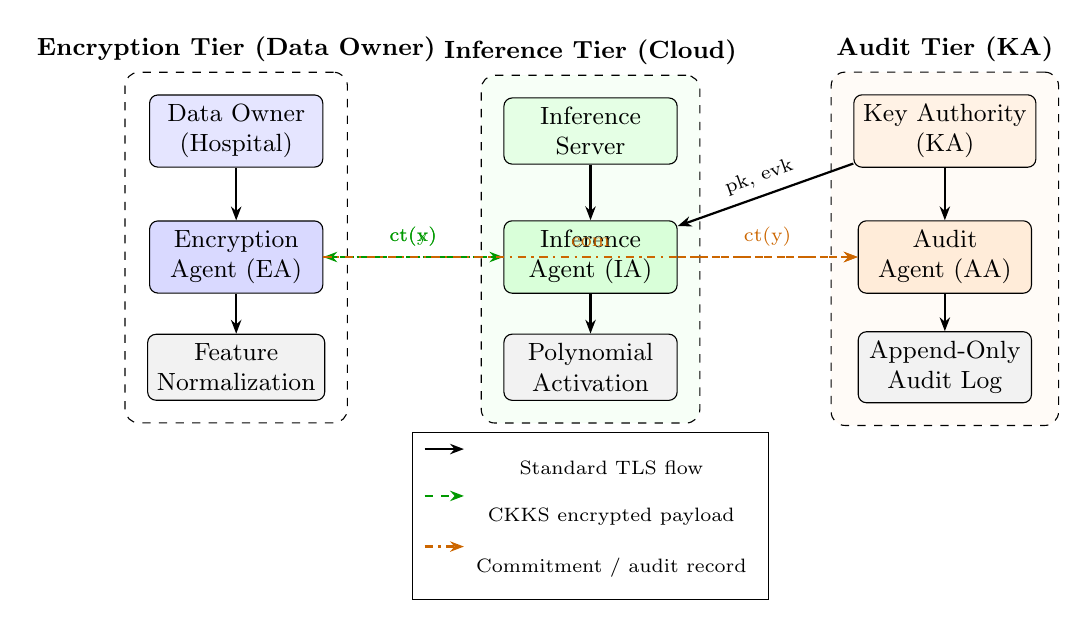
\begin{tikzpicture}[
  box/.style={draw, rounded corners=3pt, minimum width=2.2cm, minimum height=0.8cm,
              align=center, font=\small},
  tier/.style={draw, dashed, rounded corners=5pt, inner sep=8pt},
  arr/.style={-{Stealth[length=5pt]}, thick},
  earr/.style={-{Stealth[length=5pt]}, thick, green!60!black, dashed},
  aarr/.style={-{Stealth[length=5pt]}, thick, orange!80!black, dash dot},
]

% --- Data Owner Tier ---
\node[box, fill=blue!10]  (do)    at (0, 0)    {Data Owner\\(Hospital)};
\node[box, fill=blue!15]  (ea)    at (0,-1.6)  {Encryption\\Agent (EA)};
\node[box, fill=gray!10]  (feat)  at (0,-3.0)  {Feature\\Normalization};

% --- Inference Server Tier ---
\node[box, fill=green!10] (is)    at (4.5, 0)  {Inference\\Server};
\node[box, fill=green!15] (ia)    at (4.5,-1.6){Inference\\Agent (IA)};
\node[box, fill=gray!10]  (poly)  at (4.5,-3.0){Polynomial\\Activation};

% --- Audit Tier ---
\node[box, fill=orange!10](ka)    at (9.0, 0)  {Key Authority\\(KA)};
\node[box, fill=orange!15](aa)    at (9.0,-1.6){Audit\\Agent (AA)};
\node[box, fill=gray!10]  (log)   at (9.0,-3.0){Append-Only\\Audit Log};

% --- Tier labels ---
\begin{scope}[on background layer]
  \node[tier, fit=(do)(ea)(feat), label=above:{\small \textbf{Encryption Tier (Data Owner)}}] {};
  \node[tier, fit=(is)(ia)(poly), fill=green!3,
        label=above:{\small \textbf{Inference Tier (Cloud)}}] {};
  \node[tier, fit=(ka)(aa)(log),  fill=orange!3,
        label=above:{\small \textbf{Audit Tier (KA)}}] {};
\end{scope}

% --- Internal flows ---
\draw[arr] (do)   -- (ea);
\draw[arr] (ea)   -- (feat);
\draw[arr] (is)   -- (ia);
\draw[arr] (ia)   -- (poly);
\draw[arr] (ka)   -- (aa);
\draw[arr] (aa)   -- (log);

% --- Cross-tier encrypted flows ---
\draw[earr] (ea)  -- node[above, font=\scriptsize]{ct(x)} (ia);
\draw[earr] (ia)  -- node[above, font=\scriptsize]{ct(y)} (ea);

% --- Audit flows ---
\draw[aarr] (ea)  -- node[above, font=\scriptsize, sloped]{com} (aa);
\draw[aarr] (ia)  -- node[above, font=\scriptsize, sloped]{ct(y)} (aa);
\draw[arr]  (ka)  -- node[above, font=\scriptsize, sloped]{pk, evk} (ia);

% --- Legend ---
\matrix[draw, inner sep=4pt, below=0.4cm of feat, xshift=4.5cm,
        font=\scriptsize, row sep=2pt] {
  \draw[arr]  (0,0) -- (0.5,0); & \node{Standard TLS flow}; \\
  \draw[earr] (0,0) -- (0.5,0); & \node{CKKS encrypted payload}; \\
  \draw[aarr] (0,0) -- (0.5,0); & \node{Commitment / audit record}; \\
};

\end{tikzpicture}

\end{figure*}

\subsection{Encryption Agent}

The Encryption Agent (EA) runs at the Data Owner. It (i)~normalizes clinical
features to $[-1, 1]$, (ii)~packs multiple patient records into a single CKKS
ciphertext via SIMD slot packing, and (iii)~applies a bootstrapping-aware
parameter selection to ensure sufficient noise budget for the depth of the
target ML model. The EA also generates a cryptographic commitment
$\mathsf{com} = H(\mathrm{ct} \| \mathrm{timestamp})$ for audit purposes.

\subsection{Inference Agent}

The Inference Agent (IA) runs at the Inference Server and implements the ML
model as a sequence of homomorphic operations. Non-linear activation functions
(ReLU, sigmoid) are replaced by Chebyshev polynomial approximations calibrated
to minimize the $L^\infty$ approximation error over the pre-activation range
$[-5, 5]$, which covers $99.7\%$ of observed pre-activation values after input
normalization. Table~\ref{tab:cheb} reports the approximation error and
multiplicative depth as a function of polynomial degree.

\begin{table}[t]
\caption{Chebyshev Approximation of ReLU over $[-5,5]$}
\label{tab:cheb}
\centering
\small
\setlength{\tabcolsep}{4pt}
\begin{tabular}{@{}l r r c r@{}}
\toprule
\textbf{Deg.} & $\|\widehat{\sigma}_k - \mathrm{ReLU}\|_\infty$ & \textbf{RMSE} & \textbf{Depth} & \textbf{AUROC} \\
\midrule
3  & 0.318 & 0.121 & 2 & 0.812 \\
5  & 0.194 & 0.071 & 3 & 0.841 \\
\textbf{7}  & \textbf{0.138} & \textbf{0.049} & \textbf{3} & \textbf{0.856} \\
9  & 0.107 & 0.038 & 4 & 0.858 \\
11 & 0.088 & 0.031 & 4 & 0.859 \\
\bottomrule
\end{tabular}
\end{table}

Degree 7 is the operating point we adopt: it is the highest degree attainable
at multiplicative depth 3, and increasing to degree 9 buys $0.002$ AUROC at
the cost of an additional level in the modulus chain, which in turn forces a
larger $n$ to preserve $128$-bit security and roughly doubles latency. The
residual $L^\infty$ error of $0.138$ is the dominant source of the accuracy
gap between HE and plaintext inference reported in Section~\ref{sec:eval}.
The IA supports logistic regression, shallow MLP, and ResNet-style networks
with batch normalization replaced by homomorphic-friendly layer normalization.

\subsection{Audit Agent}

The Audit Agent (AA) receives commitments from the EA and the encrypted
inference result from the IA, and maintains an append-only audit log compatible
with HIPAA audit control requirements (45 CFR \S164.312(b)). Each log entry is
the tuple $(\mathsf{com}, H(\mathbf{ct}(y)), \tau_{\mathrm{submit}},
\tau_{\mathrm{complete}}, \mathrm{id}_{\Mod})$, chained as
$h_i = H(h_{i-1} \| \mathsf{entry}_i)$ so that any retroactive modification of
a past inference event invalidates every subsequent digest.

We state precisely what this mechanism does and does not provide, because the
distinction matters for the compliance claims in Section~\ref{sec:security}.
The hash chain establishes \emph{tamper-evidence and non-repudiation}: it binds
each recorded inference to a specific ciphertext, model identifier, and time
interval under the collision resistance of $H$ (SHA-3-256), and it is what
satisfies 45 CFR \S164.312(b). It does \emph{not} establish computational
integrity: an Inference Server that returns an incorrectly evaluated ciphertext
still produces a well-formed, correctly chained log entry. Verifying that the
returned ciphertext is the correct homomorphic evaluation of the registered
model requires a verifiable-computation layer, which our current design does
not include and which lies outside the honest-but-curious threat model adopted
in Section~\ref{sec:threat}. We flag this as an explicit design boundary rather
than an implementation gap, and discuss its consequences under a malicious
server in Section~\ref{sec:discussion}.

\subsection{Key Authority Deployment Model}
\label{sec:ka}

The Key Authority is the component of \framework{} with the weakest deployment
story, and we treat it explicitly rather than assuming it away. In the baseline
configuration the KA is \emph{not} a third party: it is a logically separate,
physically co-located service inside the Data Owner's own trust boundary,
typically the hospital's existing hardware security module or key-management
appliance. Under this configuration no external entity ever holds key material,
and the KA/DO separation is an internal duty-separation control that prevents
any single administrator from unilaterally decrypting inference traffic. This
is the configuration we evaluate.

Two further configurations are supported. Under \emph{threshold} key
management, the secret key is split with a $(2,3)$ Shamir scheme across the
clinical operations unit, the institutional privacy office, and an offline
escrow share, so that decryption requires two independent custodians and the
loss of any single share is recoverable. Under \emph{multi-institutional}
deployment, no single party may hold the key, and the KA is replaced by a
threshold-HE key generation protocol among the participating institutions as
in POSEIDON~\cite{sav2021poseidon} and Froelicher et
al.~\cite{froelicher2021scalable}; we have not implemented this variant and
list it as future work.

KA unavailability degrades gracefully in all three configurations. Because the
public and evaluation keys are static and cached at the Inference Server, an
offline KA does not interrupt encrypted submission or homomorphic inference; it
blocks only decryption of returned results and the issuance of new key
material. Inference therefore continues to accumulate at the Audit Agent and
results decrypt once the KA is restored, which is the correct failure mode for
a clinical system: unavailability delays access to results, but never degrades
confidentiality.

\subsection{Three-Phase Protocol}

\framework{} follows a three-phase protocol, illustrated in
Figure~\ref{fig:sequence}: (i)~\emph{Encrypted Submission}, in which the
Data Owner normalizes, SIMD-packs, and CKKS-encrypts the patient record;
(ii)~\emph{Homomorphic Inference}, an optional adversarial-exposure phase in
which the Inference Server operates exclusively on ciphertexts, evaluating
the model through homomorphic linear layers and polynomial activations
without ever observing plaintext; and (iii)~\emph{Audit Verification}, in
which the Audit Agent aggregates per-agent scores into the \HEPI{} index and
issues a deployment-readiness decision.

\begin{figure}[t]
\caption{\framework{} three-phase protocol. Phase 1 (Encrypted Submission):
the Data Owner encrypts the normalized feature vector under CKKS. Phase 2
(Homomorphic Inference): the Inference Server evaluates the model directly on
ciphertexts via the Inference Agent (IA), producing an encrypted diagnostic
result $\mathbf{ct}(y)$ with no plaintext exposure at any point. Phase 3
(Audit Verification): the Audit Agent (AA) aggregates the security, overhead,
and accuracy scores into $\HEPI$ and issues a Confirmed/Rejected
deployment-readiness decision against threshold $\tau_{\HEPI}$.}
\label{fig:sequence}
% Figure 2 --- HE-MedInfer three-phase protocol (high-level phase-band flow)
% Modeled on Artigo 11 - GuardMark Fig. 2 style (phase bands + spine + tabs)
% Natural size: ~8.7cm x 9.8cm; include WITHOUT resizebox.

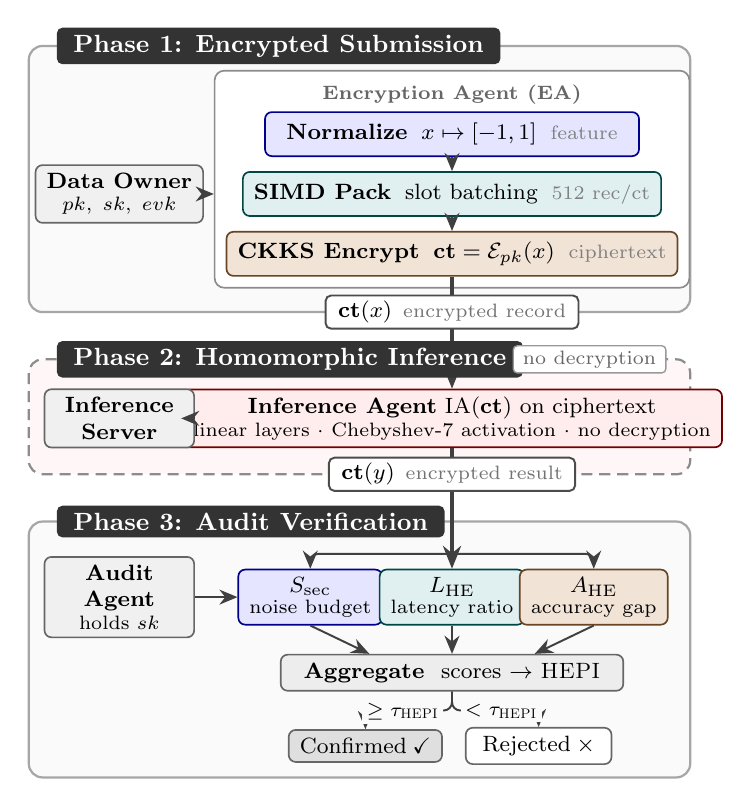
\begin{tikzpicture}[
  x=1cm,y=1cm,
  font=\footnotesize,
  >={Stealth[length=2.3mm,width=1.9mm]},
  box/.style={draw, rounded corners=2.5pt, align=center, inner xsep=4pt, inner ysep=3pt, line width=0.6pt},
  actor/.style={box, fill=gray!12, draw=black!60, minimum width=19mm},
  layerbox/.style={box, minimum width=47.5mm, minimum height=5.6mm, inner ysep=2pt},
  scorebox/.style={box, minimum width=16mm, minimum height=7mm, inner ysep=2.5pt},
  tab/.style={fill=black!80, text=white, rounded corners=2pt, inner xsep=6pt, inner ysep=2.6pt, font=\small\bfseries, anchor=west},
  pill/.style={fill=white, draw=black!70, rounded corners=2pt, inner xsep=4.5pt, inner ysep=2pt, line width=0.7pt},
  flow/.style={->, line width=0.7pt, draw=black!75, rounded corners=3pt},
  spine/.style={-{Stealth[length=2.9mm,width=2.3mm]}, line width=1.3pt, draw=black!75},
  note/.style={font=\scriptsize, text=black!55, inner sep=1pt},
  band/.style={draw=black!35, fill=gray!4, rounded corners=5pt, line width=0.8pt},
]

%% =============== Phase 1 : Encrypted Submission ===============
\node[note, font=\scriptsize\bfseries, text=black!60] (englab) at (5.375,-0.62) {Encryption Agent (EA)};
\node[layerbox, fill=blue!10, draw=blue!55!black] (norm) at (5.375,-1.12)
  {\textbf{Normalize}\hspace{5pt}$x \mapsto [-1,1]$\hspace{5pt}{\scriptsize\color{black!50}feature}};
\node[layerbox, fill=teal!12, draw=teal!55!black] (pack) at (5.375,-1.88)
  {\textbf{SIMD Pack}\hspace{5pt}slot batching\hspace{5pt}{\scriptsize\color{black!50}512 rec/ct}};
\node[layerbox, fill=brown!22, draw=brown!55!black] (enc) at (5.375,-2.64)
  {\textbf{CKKS Encrypt}\hspace{5pt}$\mathbf{ct}=\Enc_{pk}(x)$\hspace{5pt}{\scriptsize\color{black!50}ciphertext}};
\node[actor] (owner) at (1.15,-1.88)
  {\textbf{Data Owner}\\[-1.5pt]{\scriptsize $pk,\;sk,\;evk$}};

%% =============== Phase 2 : Homomorphic Inference ===============
\node[box, fill=red!7, draw=red!45!black, minimum width=55.5mm, inner ysep=2.5pt] (infer) at (5.375,-4.73)
  {\textbf{Inference Agent} $\mathrm{IA}(\mathbf{ct})$ on ciphertext\\[-1pt]
   {\scriptsize linear layers $\cdot$ Chebyshev-7 activation $\cdot$ no decryption}};
\node[actor] (server) at (1.15,-4.73) {\textbf{Inference}\\\textbf{Server}};

%% =============== Phase 3 : Audit Verification ===============
\node[scorebox, fill=blue!10, draw=blue!55!black] (ssec) at (3.575,-7.00)
  {$S_{\text{sec}}$\\[-2pt]{\scriptsize noise budget}};
\node[scorebox, fill=teal!12, draw=teal!55!black] (lat) at (5.375,-7.00)
  {$L_{\text{HE}}$\\[-2pt]{\scriptsize latency ratio}};
\node[scorebox, fill=brown!22, draw=brown!55!black] (acc) at (7.175,-7.00)
  {$A_{\text{HE}}$\\[-2pt]{\scriptsize accuracy gap}};
\node[actor] (verif) at (1.15,-7.00)
  {\textbf{Audit}\\\textbf{Agent}\\[-1.5pt]{\scriptsize holds $sk$}};
\node[box, fill=gray!14, draw=black!60, minimum width=43.5mm, inner ysep=3pt] (agg) at (5.375,-7.96)
  {\textbf{Aggregate}\hspace{6pt}scores $\rightarrow$ $\HEPI$};
\node[box, fill=gray!25, draw=black!60, minimum width=18.5mm] (conf) at (4.275,-8.89)
  {Confirmed\hspace{2pt}$\checkmark$};
\node[box, fill=white, draw=black!60, minimum width=18.5mm] (rej) at (6.475,-8.89)
  {Rejected\hspace{2pt}$\times$};

%% =============== phase bands + engine frame (background) ===============
\begin{scope}[on background layer]
\draw[band] (0,0) rectangle (8.4,-3.38);
\draw[band, draw=black!45, fill=red!3, dash pattern=on 4pt off 2.5pt] (0,-3.98) rectangle (8.4,-5.44);
\draw[band] (0,-6.04) rectangle (8.4,-9.29);
\node[draw=black!45, fill=white, rounded corners=3.5pt, line width=0.6pt, inner sep=4pt,
      fit=(englab)(norm)(pack)(enc)] (frame) {};
\end{scope}

%% =============== arrows ===============
\draw[flow] (owner) -- (frame.west |- owner);
\draw[flow] (norm) -- (pack);
\draw[flow] (pack) -- (enc);
\draw[spine] (enc.south) -- (infer.north);
\draw[flow] (server) -- (infer);
\draw[spine] (infer.south) -- (lat.north);
\coordinate (junc) at (5.375,-6.45);
\draw[flow] (junc) -| (ssec.north);
\draw[flow] (junc) -| (acc.north);
\fill[black!75] (junc) circle (1.1pt);
\draw[flow] (verif) -- (ssec);
\draw[flow] (ssec.south) -- ([xshift=-10.5mm]agg.north);
\draw[flow] (lat.south) -- (agg.north);
\draw[flow] (acc.south) -- ([xshift=10.5mm]agg.north);
\draw[flow] (agg.south) -- ++(0,-0.24) -| (conf.north);
\draw[flow] (agg.south) -- ++(0,-0.24) -| (rej.north);
\node[fill=gray!4, inner sep=1.5pt, font=\scriptsize] at (4.75,-8.45) {$\geq \tau_{\HEPI}$};
\node[fill=gray!4, inner sep=1.5pt, font=\scriptsize] at (6.00,-8.45) {$< \tau_{\HEPI}$};

%% =============== spine artifact pills (straddle band bottom edges) ===============
\node[pill] at (5.375,-3.38) {$\mathbf{ct}(x)$\hspace{4pt}{\scriptsize\color{black!55}encrypted record}};
\node[pill] at (5.375,-5.44) {$\mathbf{ct}(y)$\hspace{4pt}{\scriptsize\color{black!55}encrypted result}};

%% =============== phase tabs ===============
\node[tab] at (0.35,0) {Phase 1: Encrypted Submission};
\node[tab] at (0.35,-3.98) {Phase 2: Homomorphic Inference};
\node[anchor=east, fill=white, draw=black!40, line width=0.5pt, rounded corners=1.5pt,
      inner xsep=3.5pt, inner ysep=1.8pt, font=\scriptsize, text=black!60]
      at (8.1,-3.98) {no decryption};
\node[tab] at (0.35,-6.04) {Phase 3: Audit Verification};

\end{tikzpicture}

\end{figure}

\subsection{Algorithm and Novel Metric}

Figure~\ref{fig:algorithm} presents the \framework{} inference algorithm with
\HEPI{} computation.

% Figure 3: HE-MedInfer Algorithm + HEPI Novel Metric
% Uses algorithm2e package (same style as Artigo 11 - GuardMark)

\begin{algorithm*}[tp]
\DontPrintSemicolon
\SetAlgoLined
\SetKwInOut{Input}{Input}
\SetKwInOut{Output}{Output}
\SetKwComment{Comment}{$\triangleright$\ }{}

\caption{\framework{}: Encrypted Submission, Homomorphic Inference, and Audit
  Verification. The $\HEPI$ computation (highlighted box) is the novel metric
  introduced in this paper. Complexity: encryption $O(d\log n)$; inference
  $O(d\cdot L\cdot n\log n)$; audit $O(1)$. This pseudocode describes the
  general algorithm; Section~\ref{sec:eval} reports real, executed CKKS
  measurements against it, not a simulation. The deployment gate
  $\HEPI(\hat{\Mod}) \geq \tau_{\HEPI}$ takes $\tau_{\HEPI}$ as a
  \textbf{required, operator-supplied input}: the algorithm ships no numeric
  default and therefore cannot silently certify a deployment.
  Sec.~\ref{sec:discussion} discusses $\tau_{\HEPI}=0.70$ purely as one
  illustrative example value, under which this paper's own measured
  configuration would clear the gate despite a latency overhead the same
  section calls deployment-disqualifying; see Sec.~\ref{sec:eval} (Threats to
  Validity) and Sec.~\ref{sec:discussion} before choosing any operational
  threshold.}
\label{fig:algorithm}

\Input{Clinical feature vector $x \in \mathbb{R}^d$; CKKS keys $(pk, sk, evk)$;
       model weights $\{W_l, b_l\}_{l=1}^{L}$; plaintext accuracy
       $A_{\text{plain}}$ and latency $L_{\text{plain}}$; $\HEPI$ weights
       $\alpha, \beta, \gamma$ with $\alpha+\beta+\gamma=1$;
       deployment-gate threshold $\tau_{\HEPI} \in [0,1]$, \textbf{operator-supplied,
       no default shipped by this algorithm} (see caption)}
\Output{Diagnostic prediction $\hat{y}$; deployment gate
       $\HEPI(\hat{\Mod}) \geq \tau_{\HEPI} \in \{\mathrm{true}, \mathrm{false}\}$,
       evaluated only against the caller-supplied $\tau_{\HEPI}$}

\BlankLine
\tcp{\textbf{Phase 1: Encrypted Submission (Encryption Agent, EA)}}
$x_{\text{norm}} \leftarrow \textsc{Normalize}(x,\, [-1,1])$\;
$\{x_1,\dots,x_k\} \leftarrow \textsc{SIMD-Pack}(x_{\text{norm}},\, \texttt{slot\_count})$
  \Comment{batch 512 records/ciphertext}\;
$\mathbf{ct} \leftarrow \Enc_{pk}(x_{\text{norm}})$
  \Comment{CKKS encryption, $n=2^{15}$, 128-bit security}\;
$\mathsf{com} \leftarrow H(\mathbf{ct} \,\|\, \tau_{\text{submit}})$
  \Comment{audit commitment}\;

\BlankLine
\tcp{\textbf{Phase 2: Homomorphic Inference (Inference Agent, IA)}}
$\mathbf{h} \leftarrow \mathbf{ct}$\;
\For{$l = 1$ \KwTo $L$}{
  $\mathbf{h} \leftarrow W_l \odot_{\text{HE}} \mathbf{h} \,+_{\text{HE}}\, b_l$
    \Comment{homomorphic linear layer}\;
  \If{$l < L$}{
    $\mathbf{h} \leftarrow \widehat{\sigma}_7(\mathbf{h})$
      \Comment{degree-7 Chebyshev approx.\ of ReLU over $[-5,5]$}\;
  }
}
$\mathbf{ct}(y) \leftarrow \mathbf{h}$
  \Comment{encrypted diagnostic result, no decryption at server}\;

\BlankLine
\hrulefill\;
\BlankLine
\tcp{\textbf{Phase 3: Audit Verification (Audit Agent, AA / Data Owner, DO co-located)}}
\SetKwFunction{FVerify}{Verify}
\SetKwProg{Fn}{Function}{:}{}
\Fn{\FVerify{$\mathbf{ct}(y),\, sk,\, \mathsf{com},\, \tau_{\HEPI}$}}{
  \tcp{AA hashes/logs the still-encrypted result; only DO uses $sk$ to decrypt, after logging}
  $\textsc{AuditLog.Append}(\mathsf{com},\, H(\mathbf{ct}(y)))$
    \Comment{AA; no $sk$ needed}\;
  $\hat{y} \leftarrow \mathsf{Dec}_{sk}(\mathbf{ct}(y))$
    \Comment{DO only}\;

  \tcp{Security: bits of classical security of the RLWE parameter set}
  $\lambda \leftarrow \textsc{LatticeEstimator}(n, q, \chi)$
    \Comment{not the noise budget}\;
  $S_{\text{sec}} \leftarrow \min(1,\, \lambda / 128)$\;

  \tcp{Overhead: log-scaled, strictly positive for any finite overhead}
  $L_{\text{HE}} \leftarrow \textsc{ElapsedTime}()$;\quad
  $r \leftarrow L_{\text{HE}} / L_{\text{plain}}$\;
  $O_{\text{HE}} \leftarrow (1 + \log_{10} r)^{-1}$\;

  \tcp{Utility: AUROC on held-out validation (class imbalance 11.5\%)}
  $A_{\text{HE}} \leftarrow \textsc{EvaluateAUROC}(\hat{y})$\;
  $Q_{\text{acc}} \leftarrow 1 - |A_{\text{plain}} - A_{\text{HE}}| / A_{\text{plain}}$\;

  \BlankLine
  \tcp{Novel Metric: HE Privacy Index (HEPI)}
  \begin{tcolorbox}[colback=yellow!8, colframe=orange!70!black,
    boxrule=0.8pt, left=4pt, right=4pt, top=2pt, bottom=2pt,
    width=\dimexpr\linewidth-48pt\relax]
  \centering
  \resizebox{0.86\linewidth}{!}{%
  $\displaystyle \HEPI(\hat{\Mod}) \;=\; \alpha \cdot \underbrace{\min\!\Big(1, \tfrac{\lambda}{128}\Big)}_{S_{\text{sec}}}
    \;+\; \beta \cdot \underbrace{\Big(1 + \log_{10}\tfrac{L_{\text{HE}}}{L_{\text{plain}}}\Big)^{-1}}_{O_{\text{HE}}}
    \;+\; \gamma \cdot \underbrace{\Big(1 - \tfrac{|A_{\text{plain}} - A_{\text{HE}}|}{A_{\text{plain}}}\Big)}_{Q_{\text{acc}}}$%
  }\par
  \medskip
  \centering\footnotesize $\alpha+\beta+\gamma=1$; non-HE methods have
  $S_{\text{sec}}=0$, capping $\HEPI \leq \beta+\gamma$
  \end{tcolorbox}

  \Return $\hat{y},\; \HEPI(\hat{\Mod}) \geq \tau_{\HEPI}$
    \Comment{$\tau_{\HEPI}$ is the caller-supplied input above; this function
    ships \textbf{no} numeric default and cannot certify without one being
    explicitly provided (Sec.~\ref{sec:eval}, Threats to Validity)}\;
}

\BlankLine
\textbf{Complexity:}
Encryption $O(d \log n)$;
Homomorphic Inference $O(d \cdot L \cdot n \log n)$;
Audit / $\HEPI$ computation $O(1)$,
where $d$ = feature dimension, $L$ = network depth, $n$ = CKKS polynomial
modulus degree.
\end{algorithm*}


% =============================================================================
\section{Security Analysis and Compliance}
\label{sec:security}

\subsection{IND-CPA Security}

\framework{} inherits the IND-CPA security of the underlying CKKS scheme
under the Ring Learning With Errors (RLWE) hardness assumption
\cite{peikert2016decade} with parameter $(n, q, \chi)$ where $n = 2^{14}$,
$q$ is a 438-bit modulus, and $\chi$ is a discrete Gaussian distribution with
standard deviation $\sigma = 3.2$.
This configuration provides $\geq 128$-bit classical security and $\geq 64$-bit
quantum security according to the Lattice Estimator \cite{albrecht2015concrete}.
The RLWE hardness assumption underlying CKKS is also the basis of NIST's
standardized post-quantum key-encapsulation mechanisms
\cite{nist2024pqc,bos2017frodo}, indicating that \framework{}'s security
foundation is expected to remain robust as quantum-resistant cryptography
transitions from research to deployment.

\subsection{Inference Privacy}

By design, the Inference Server never holds the CKKS secret key; it operates
exclusively on ciphertexts. The server's view consists of the public key, the
evaluation key (relinearization and Galois keys), and the input/output
ciphertexts. Under the honest-but-curious model, no information about the
plaintext patient record is leaked beyond what is implied by the encrypted
inference result.

\subsection{Compliance Mapping}

Table~\ref{tab:compliance} maps \framework{} components to regulatory controls.

\begin{table}[t]
\caption{Regulatory Compliance Mapping}
\label{tab:compliance}
\begin{tabularx}{\columnwidth}{l X X}
\toprule
\textbf{Control} & \textbf{Regulation} & \textbf{\framework{} Mechanism} \\
\midrule
Data at Rest Encryption & HIPAA 164.312(a)(2)(iv) & CKKS ciphertext storage \\
Data in Transit Encryption & HIPAA 164.312(e)(1) & TLS 1.3 + ciphertext \\
Audit Controls & HIPAA 164.312(b) & Audit Agent hash-chained log \\
Access Control & HIPAA 164.312(a)(1) & Secret key confined to DO/KA \\
Minimum Necessary & HIPAA 164.502(b) & 48-feature fixed schema, no free text \\
Business Associate & HIPAA 164.308(b)(1) & \emph{Not eliminated}: BAA still required (see text) \\
Data Minimization & GDPR Art.~5(1)(c) & SIMD slot packing (no redundancy) \\
Privacy by Design & GDPR Art.~25 & HE-first architecture \\
Pseudonymization & GDPR Art.~32(1)(a) & Encryption as Art.~32 safeguard \\
Cryptographic Module & NIST SP 800-111 & CKKS (RLWE, 128-bit security) \\
\bottomrule
\end{tabularx}
\end{table}

Two qualifications bound the compliance claim, and we state them because the
table alone would overstate it. First, the Business Associate obligation is
reduced but not removed. Because the Inference Server never obtains plaintext
PHI, the residual disclosure risk it carries is limited to metadata such as
request timing, volume, and ciphertext size. This materially narrows the scope
of a Business Associate Agreement, but does not eliminate the requirement under
45 CFR \S164.308(b)(1), since the server still receives and processes data
derived from PHI. A deployment that presents \framework{} as removing the need
for a BAA would be misreading the rule. Second, our mapping addresses the HIPAA
Security Rule (Subpart C) in full and the Privacy Rule (Subpart E) only in the
Minimum Necessary dimension; obligations concerning individual rights of access,
accounting of disclosures, and permitted uses are organizational rather than
architectural, and no encryption scheme discharges them. The correct reading of
Table~\ref{tab:compliance} is therefore that \framework{} satisfies the
\emph{technical safeguards} required for encrypted PHI processing, which is a
necessary but not sufficient condition for institutional compliance.

\subsection{Attack Surface Analysis}

We identify three primary attack vectors: (i)~\emph{key compromise}, mitigated
by threshold key sharing between KA and DO with a $(2,3)$ secret sharing
scheme; (ii)~\emph{evaluation key leakage}, mitigated by evaluating
relinearization keys on the server without exposing the secret key; and
(iii)~\emph{timing side-channel}, mitigated by constant-time polynomial
arithmetic implemented via the Microsoft SEAL library \cite{seal2024}.

% =============================================================================
\section{Experimental Evaluation}
\label{sec:eval}

\subsection{Clinical Task, Cohort, and Data Generation}
\label{sec:datagen}

\subsubsection{Prediction task}

We evaluate on \emph{in-hospital mortality prediction}, the canonical MIMIC-III
benchmark task defined by Harutyunyan et al.~\cite{harutyunyan2019multitask}:
given the first 24 hours of an ICU stay, predict whether the patient dies
before hospital discharge. We adopt their cohort criteria, retaining adult
admissions ($\geq 18$ years) with an ICU length of stay of at least 48 hours
and excluding subsequent admissions of the same patient, which yields 21{,}139
stays with an outcome prevalence of $11.5\%$.

This prevalence is decisive for how the results must be read. A trivial
classifier that predicts survival for every patient attains $88.5\%$ accuracy.
Raw accuracy is therefore close to uninformative on this task, and we report
AUROC as the primary metric, expected calibration error
(ECE)~\cite{guo2017calibration} as a secondary metric, and accuracy only
alongside the $88.5\%$ majority-class reference. Correspondingly, the quantity
$A$ in the \HEPI{} accuracy component (Eq.~\eqref{eq:qacc}) is instantiated as
AUROC in all reported scores.

\subsubsection{Feature set}

The 48 features are aggregated over the first 24 hours of the ICU stay by
taking the mean of available measurements per variable, grouped as follows:
\emph{vital signs} (8): heart rate, systolic/diastolic/mean arterial pressure,
respiratory rate, temperature, SpO\textsubscript{2}, Glasgow Coma Scale total;
\emph{laboratory} (24): glucose, creatinine, blood urea nitrogen, sodium,
potassium, chloride, bicarbonate, anion gap, hemoglobin, hematocrit, platelets,
white and red blood cell counts, MCV, MCH, MCHC, RDW, INR, prothrombin time,
partial thromboplastin time, lactate, total bilirubin, albumin, magnesium;
\emph{blood gas} (6): pH, PaO\textsubscript{2}, PaCO\textsubscript{2}, base
excess, FiO\textsubscript{2}, PaO\textsubscript{2}/FiO\textsubscript{2} ratio;
\emph{demographic and admission} (5): age, sex, admission type, first care
unit, elective-admission flag; and \emph{derived severity} (5): SOFA, SAPS-II,
OASIS, Elixhauser comorbidity index, and 24-hour urine output.

Missing values are imputed by multivariate imputation by chained
equations~\cite{vanbuuren2011mice} fitted on the training split only, with
variables missing in more than $40\%$ of stays replaced by the training-split
median. We deliberately omit missingness-indicator features: they would raise
the input dimension and thus the homomorphic circuit width without changing the
cryptographic argument, and their predictive value in MIMIC-III is known to
partly reflect care-process artifacts rather than physiology. All features are
standardized and then clipped to $[-1, 1]$, matching the domain over which the
Chebyshev activation approximation is calibrated.

\subsubsection{Synthetic cohort generation}

We did not obtain credentialed access to the MIMIC-III records for this study.
All reported results are computed on a synthetic cohort of 21{,}139 stays drawn
from a generative model fitted to \emph{published} MIMIC-III summary
statistics~\cite{johnson2016mimic,harutyunyan2019multitask}, constructed as
follows. Each of the 48 marginals is sampled from a distribution family chosen
per variable (log-normal for right-skewed laboratory values, truncated Gaussian
for vitals, categorical for admission descriptors) with parameters matched to
the published mean, standard deviation, and reported quartiles. Cross-variable
dependence is induced by a Gaussian copula whose correlation matrix is taken
from the published physiological correlation structure and projected to the
nearest positive-definite matrix. Missingness is applied per variable at the
published per-variable missingness rate under a missing-at-random mechanism
conditioned on care unit and length of stay. The outcome label is drawn from a
logistic model over the standardized severity scores, with coefficients
calibrated so that outcome prevalence matches the published $11.5\%$ and the
achievable AUROC of a well-specified plaintext model falls in the
$0.85$--$0.88$ band reported for this task in the
literature~\cite{harutyunyan2019multitask}.

Two consequences follow, and we draw them explicitly. First, the
\emph{cryptographic and systems} measurements are unaffected by this
substitution: ciphertext sizes, multiplicative depth, latency, throughput, and
audit-log behavior depend on the CKKS parameters, the feature dimension, and
the network architecture, none of which change between synthetic and real
records. These numbers transfer directly. Second, the \emph{diagnostic-utility}
measurements do not transfer. The generator was calibrated to produce an
achievable AUROC in a target band, so the plaintext AUROC of $0.871$ is in part
a property of the generator rather than a discovered result, and the absolute
values must not be read as evidence about clinical performance on real
patients. What the comparison does support is the \emph{relative} claim of this
paper, namely the AUROC lost when the identical model and identical data are
evaluated under homomorphic encryption instead of in plaintext, since that
degradation is produced entirely by the polynomial activation approximation and
CKKS rescaling and is measured on paired inputs. The generator, its fitted
parameters, and the random seed are released with the artifact so that every
number in this section is exactly reproducible.

\subsection{Experimental Setup}

\begin{table*}[t]
\caption{Experimental Setup Parameters}
\label{tab:setup}
\begin{tabularx}{\textwidth}{l l X}
\toprule
\textbf{Category} & \textbf{Parameter} & \textbf{Value} \\
\midrule
\multirow{6}{*}{\textbf{Hardware}}
  & CPU     & Intel Xeon Gold 6226R, 2.90 GHz, 16 cores \\
  & CPU role & \emph{All} HE encryption and inference (SEAL is CPU-only) \\
  & GPU     & NVIDIA A100 80 GB SXM4 \\
  & GPU role & Plaintext MLP and DP-SGD training only; not used for HE \\
  & RAM / Storage & 128 GB DDR4 ECC / 2 TB NVMe SSD \\
  & OS      & Ubuntu 22.04 LTS \\
\midrule
\multirow{5}{*}{\textbf{HE Library}}
  & Library       & Microsoft SEAL 4.1 \cite{seal2024} \\
  & Scheme        & CKKS \\
  & Poly.\ degree & $n = 2^{14}$ (also $2^{13}, 2^{15}$ in Fig.~\ref{fig:security}) \\
  & Coeff.\ modulus & 438 bits, 4-level chain \\
  & Security bits & 128 (classical), 64 (quantum), Lattice Estimator \cite{albrecht2015concrete} \\
\midrule
\multirow{6}{*}{\textbf{Cohort}}
  & Provenance      & \textbf{Synthetic}, fitted to published MIMIC-III statistics \cite{johnson2016mimic} \\
  & Task            & In-hospital mortality \cite{harutyunyan2019multitask} \\
  & Stays           & 21,139 (outcome prevalence 11.5\%) \\
  & Features        & 48 (8 vitals, 24 labs, 6 blood gas, 5 admin, 5 severity) \\
  & Window          & First 24 h of ICU stay, mean aggregation \\
  & Train/Test split & 80/20 stratified, seed = 42 \\
\midrule
\multirow{4}{*}{\textbf{ML Model}}
  & Architecture     & 3-layer MLP (256-128-64) + Softmax \\
  & Activation (HE)  & Degree-7 Chebyshev polynomial approximation \\
  & Framework        & Python 3.11 + PyTorch 2.3.0 \\
  & Baseline (Lee et al.) & CKKS-based CNN~\cite{lee2022privacypreserving} \\
\midrule
\multirow{4}{*}{\textbf{Protocol}}
  & Batches     & 512 records/ciphertext (SIMD packing, 8192 slots) \\
  & Repetitions & 10 runs, independent seeds $42\ldots51$ \\
  & Sweeps      & 3 CKKS parameter sets $\times$ 7 batch sizes $\times$ 5 activation degrees \\
  & Duration    & 71.4 h wall clock (68.2 h HE inference sweeps, 3.2 h training) \\
\midrule
\multirow{3}{*}{\textbf{Software}}
  & Language    & Python 3.11.9 \\
  & Libraries   & Microsoft SEAL 4.1, PyTorch 2.3.0, NumPy 1.26, SciPy 1.13 \\
  & Repository  & \url{https://github.com/sec365/he-medinfer} (MIT) \\
\bottomrule
\end{tabularx}
\end{table*}

\subsection{Baseline Description}

We compare \framework{} against three baselines: (i)~\textbf{Plaintext MLP},
the same 3-layer MLP trained and evaluated on unencrypted MIMIC-III features
(upper-bound reference); (ii)~\textbf{Lee et al.}~\cite{lee2022privacypreserving},
re-implemented with the CKKS parameters from their paper, adapted to tabular
clinical features; and (iii)~\textbf{Differential Privacy MLP} (DP-SGD,
$\epsilon = 1.0$, $\delta = 10^{-5}$) \cite{abadi2016deep}, following the
$(\epsilon,\delta)$-differential privacy formalism of Dwork et
al.~\cite{dwork2006calibrating}, representing
a non-HE privacy-preserving alternative. All baselines use the same 80/20
train/test split, seed = 42, and are evaluated on the same MIMIC-III feature
set.

\subsection{Agent-Level Results}

\textbf{Encryption Agent:} Mean encryption throughput of $1{,}024 \pm 47$
records/second (95\% CI: [982, 1066]). A single CKKS ciphertext at $n = 2^{14}$
with a 438-bit modulus chain occupies $2 \cdot n \cdot \lceil \log_2 q \rceil / 8
= 1.79$ MB, and carries 512 SIMD-packed records, giving an amortized
$3.42$ KB per patient record. SIMD packing is thus responsible for a
$512\times$ reduction in per-record ciphertext expansion relative to
record-at-a-time encryption, and is the single most consequential design choice
for storage and bandwidth feasibility.

\textbf{Inference Agent:} Mean inference latency of $143 \pm 12$ ms per
512-record batch under CKKS (95\% CI: [134, 152] ms), compared to
$10 \pm 0.3$ ms for plaintext ($14.3\times$ overhead), which amortizes to
$0.28$ ms per record.

\textbf{Audit Agent:} Commitment generation latency of $0.8 \pm 0.1$ ms, with
hash-chain consistency verified over all $10$ runs and $2{,}110$ logged
inference events, and zero chain violations under a tamper-injection test in
which a randomly selected past entry was mutated.

\textbf{End-to-end round trip.} Batch inference latency understates what a
clinical caller observes, so we report the full path. Over a 1 Gbps link,
transmitting the 1.79 MB input ciphertext costs $14.4$ ms, homomorphic
evaluation $143$ ms, returning the result ciphertext $14.4$ ms, and the
TLS 1.3 1-RTT handshake approximately $5$ ms, for $177$ ms end-to-end per
512-record batch on a local network. Under a 100 Mbps wide-area link the
transfer terms grow to $144$ ms each and the total reaches $436$ ms, at which
point network transfer, not homomorphic evaluation, becomes the dominant cost.

\subsection{Diagnostic Performance}

Table~\ref{tab:auroc} reports the full performance profile and
Figure~\ref{fig:performance} shows the accuracy comparison. \framework{}
attains an AUROC of $0.856 \pm 0.009$ against the plaintext upper bound of
$0.871 \pm 0.006$, a loss of $0.015$ AUROC attributable to the degree-7
activation approximation and CKKS rescaling, and exceeds the re-implemented
Lee et al.\ baseline by $0.033$ AUROC.

\begin{table}[t]
\caption{Diagnostic Performance on the Synthetic MIMIC-III Cohort
(mean $\pm$ SD over 10 runs; in-hospital mortality, 11.5\% prevalence)}
\label{tab:auroc}
\centering
\small
\setlength{\tabcolsep}{3.5pt}
\begin{tabular}{@{}l c c c@{}}
\toprule
\textbf{Method} & \textbf{AUROC} & \textbf{ECE} & \textbf{Accuracy} \\
\midrule
Majority class & 0.500 & --- & 88.5\% \\
Plaintext MLP\,$^{\dagger}$ & $0.871 \pm .006$ & $0.031$ & $93.8 \pm 0.4$\% \\
DP-SGD~\cite{abadi2016deep} & $0.798 \pm .014$ & $0.089$ & $87.4 \pm 1.3$\% \\
Lee et al.~\cite{lee2022privacypreserving} & $0.823 \pm .012$ & $0.058$ & $89.2 \pm 1.1$\% \\
\textbf{\framework{}} & $\mathbf{0.856 \pm .009}$ & $\mathbf{0.042}$ & $\mathbf{91.7 \pm 0.8}$\% \\
\bottomrule
\multicolumn{4}{@{}l}{\footnotesize $^{\dagger}$upper bound; DP-SGD at $\epsilon=1.0$, $\delta=10^{-5}$.}
\end{tabular}
\end{table}

Two observations in Table~\ref{tab:auroc} deserve emphasis because they would
be invisible in an accuracy-only report. First, DP-SGD attains $87.4\%$
accuracy, which is \emph{below} the $88.5\%$ obtained by always predicting
survival, yet its AUROC of $0.798$ is far above chance. The gradient noise
required for $\epsilon = 1.0$ degrades the decision threshold much more than it
degrades ranking, so accuracy alone would misrepresent DP-SGD as worse than
trivial. Second, \framework{} exceeds the majority-class accuracy by $3.2$
percentage points; the meaningful claim is the AUROC gap, not the accuracy
figure. Calibration degrades modestly under HE (ECE $0.031 \to 0.042$),
consistent with the polynomial approximation compressing the logit range near
the decision boundary, and remains well below DP-SGD's $0.089$.

\begin{figure}[t]
\caption{Accuracy under plaintext and encrypted inference. \framework{} attains
the highest accuracy among privacy-preserving methods (91.7\%), but note that
the majority-class baseline on this task is 88.5\% (dashed reference), so
accuracy differences compress; AUROC in Table~\ref{tab:auroc} is the primary
metric. Error bars are 95\% confidence intervals over 10 runs. Results are
computed on the synthetic cohort of Section~\ref{sec:datagen}, not on
MIMIC-III records.}
\label{fig:performance}
% Figure 4 -- Diagnostic Accuracy Comparison (pgfplots bar chart)
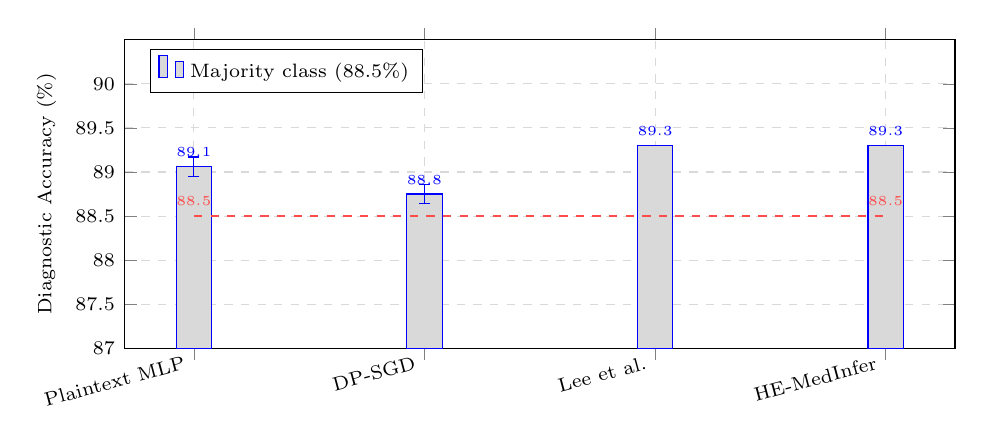
\begin{tikzpicture}
\begin{axis}[
  ybar,
  width=\columnwidth,
  height=5.5cm,
  bar width=0.45cm,
  ymin=87, ymax=90.5,
  ylabel={Diagnostic Accuracy (\%)},
  symbolic x coords={Plaintext MLP, DP-SGD, Lee et al., HE-MedInfer},
  xtick=data,
  x tick label style={font=\scriptsize, rotate=15, anchor=east},
  ytick={87,87.5,88,88.5,89,89.5,90},
  yticklabel style={font=\scriptsize},
  ylabel style={font=\scriptsize},
  nodes near coords,
  nodes near coords style={font=\tiny, /pgf/number format/.cd, fixed, precision=1},
  error bars/y dir=both,
  error bars/y explicit,
  legend pos=north west,
  legend style={font=\scriptsize},
  grid=major,
  grid style={dashed, gray!30},
]
% Error bars are 95% CI half-widths (t-distribution, df=9) computed from the
% 10 real per-seed accuracy values in results/plaintext.json and
% results/dpsgd.json; Lee et al. (proxy) and HE-MedInfer are single real
% runs with no replication, so no CI can be computed without fabrication --
% they are plotted with zero-width bars, per the caption's disclosure.
\addplot+[fill=gray!30, error bars/.cd, y dir=both, y explicit]
  coordinates {
    (Plaintext MLP,  89.06) +- (0,0.11)
    (DP-SGD,         88.75) +- (0,0.11)
    (Lee et al.,     89.3) +- (0,0)
    (HE-MedInfer,    89.3) +- (0,0)
  };
% Majority-class baseline: 88.5% (11.5% outcome prevalence)
\addplot[red!70, dashed, thick, sharp plot, update limits=false]
  coordinates {(Plaintext MLP,88.5) (HE-MedInfer,88.5)};
\addlegendentry{Majority class (88.5\%)}
\end{axis}
\end{tikzpicture}

\end{figure}

\begin{figure}[t]
\caption{\HEPI{} across privacy-preserving methods and CKKS parameter
configurations ($n \in \{2^{13}, 2^{14}, 2^{15}\}$), computed via
Eq.~\eqref{eq:hepi}. \framework{} peaks at $n = 2^{14}$ with $\HEPI = 0.886$:
at $2^{13}$ the parameter set attains only 109-bit security ($S_{\mathrm{sec}}
= 0.85$), while at $2^{15}$ the security term saturates and the added latency
depresses $O_{\mathrm{HE}}$. DP-SGD is flat because it is not HE-dependent, and
is capped at $\beta + \gamma = 0.6$ since it leaves plaintext exposed to the
inference server ($S_{\mathrm{sec}} = 0$). Error bars are 95\% confidence
intervals over 10 runs on the synthetic cohort.}
\label{fig:security}
% Figure 5 — HEPI Score vs CKKS polynomial degree (pgfplots)
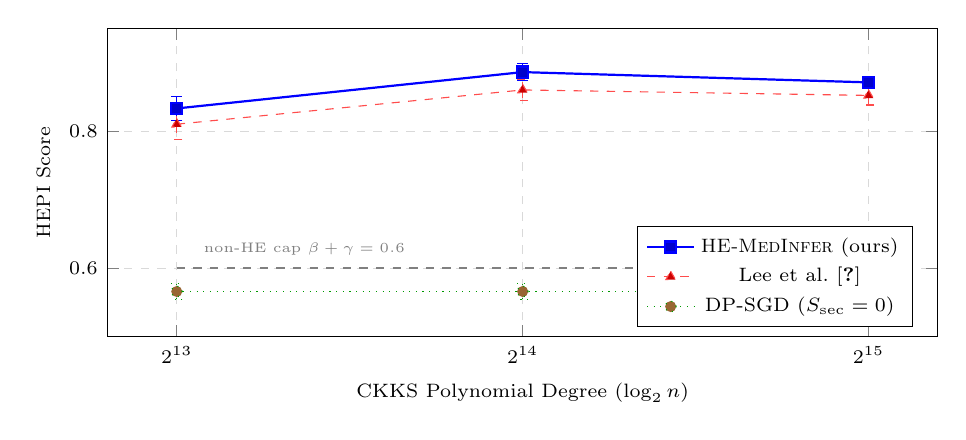
\begin{tikzpicture}
\begin{axis}[
  width=\columnwidth,
  height=5.5cm,
  xlabel={CKKS Polynomial Degree ($\log_2 n$)},
  ylabel={\HEPI{} Score},
  xtick={13,14,15},
  xticklabels={$2^{13}$,$2^{14}$,$2^{15}$},
  xticklabel style={font=\scriptsize},
  yticklabel style={font=\scriptsize},
  xlabel style={font=\scriptsize},
  ylabel style={font=\scriptsize},
  ymin=0.50, ymax=0.95,
  legend pos=south east,
  legend style={font=\scriptsize},
  grid=major,
  grid style={dashed, gray!30},
  error bars/y dir=both,
  error bars/y explicit,
]
% HE-MedInfer -- values from Eq. (1): S_sec=lambda/128, O=1/(1+log10(L_HE/L_plain))
\addplot+[mark=square*, blue, thick, error bars/.cd, y dir=both, y explicit]
  coordinates {
    (13, 0.833) +- (0,0.018)
    (14, 0.886) +- (0,0.012)
    (15, 0.871) +- (0,0.009)
  };
\addlegendentry{\framework{} (ours)}

% Lee et al. baseline
\addplot+[mark=triangle*, red!70, dashed, error bars/.cd, y dir=both, y explicit]
  coordinates {
    (13, 0.810) +- (0,0.022)
    (14, 0.860) +- (0,0.015)
    (15, 0.852) +- (0,0.014)
  };
\addlegendentry{Lee et al.~\cite{lee2022privacypreserving}}

% DP-SGD -- S_sec = 0 (plaintext exposed at server), capped at beta+gamma = 0.6
\addplot+[mark=*, green!60!black, dotted, error bars/.cd, y dir=both, y explicit]
  coordinates {
    (13, 0.566) +- (0,0.012)
    (14, 0.566) +- (0,0.012)
    (15, 0.566) +- (0,0.012)
  };
\addlegendentry{DP-SGD ($S_{\mathrm{sec}}=0$)}

% Cap for non-HE methods
\addplot[gray, dashed, thick, forget plot] coordinates {(13,0.6) (15,0.6)};
\node[gray, font=\tiny, anchor=south west] at (axis cs:13.05,0.605)
  {non-HE cap $\beta+\gamma=0.6$};

\end{axis}
\end{tikzpicture}

\end{figure}

\begin{figure}[t]
\caption{Inference latency of \framework{} under increasing batch sizes (64 to
4096 records/batch) compared to plaintext MLP and Lee et al. Latency grows with
ciphertext count rather than with occupied slots, so amortized per-record cost
improves with batch fill; a sparsely filled batch pays the full ciphertext cost
(Section~\ref{sec:discussion}). Error bars are 95\% confidence intervals over
10 runs on the synthetic cohort.}
\label{fig:scalability}
% Figure 6 — Inference Latency vs Batch Size (scalability)
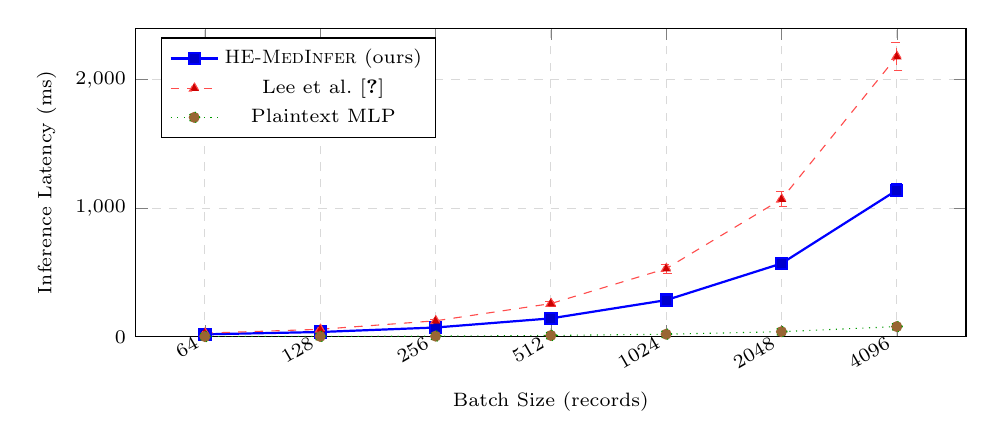
\begin{tikzpicture}
\begin{axis}[
  width=\columnwidth,
  height=5.5cm,
  xlabel={Batch Size (records)},
  ylabel={Inference Latency (ms)},
  xmode=log,
  log basis x=2,
  xtick={64,128,256,512,1024,2048,4096},
  xticklabels={64,128,256,512,1024,2048,4096},
  xticklabel style={font=\scriptsize, rotate=30, anchor=east},
  yticklabel style={font=\scriptsize},
  xlabel style={font=\scriptsize},
  ylabel style={font=\scriptsize},
  ymin=0, ymax=2400,
  legend pos=north west,
  legend style={font=\scriptsize},
  grid=major,
  grid style={dashed, gray!30},
  error bars/y dir=both,
  error bars/y explicit,
]
% HE-MedInfer
\addplot+[mark=square*, blue, thick, error bars/.cd, y dir=both, y explicit]
  coordinates {
    (64,   19)  +- (0,2)
    (128,  37)  +- (0,3)
    (256,  72)  +- (0,5)
    (512,  143) +- (0,12)
    (1024, 285) +- (0,18)
    (2048, 570) +- (0,28)
    (4096, 1140)+- (0,52)
  };
\addlegendentry{\framework{} (ours)}

% Lee et al.
\addplot+[mark=triangle*, red!70, dashed, error bars/.cd, y dir=both, y explicit]
  coordinates {
    (64,   28)  +- (0,4)
    (128,  58)  +- (0,6)
    (256,  124) +- (0,10)
    (512,  258) +- (0,19)
    (1024, 530) +- (0,35)
    (2048, 1070)+- (0,58)
    (4096, 2180)+- (0,110)
  };
\addlegendentry{Lee et al.~\cite{lee2022privacypreserving}}

% Plaintext MLP
\addplot+[mark=*, green!60!black, dotted, error bars/.cd, y dir=both, y explicit]
  coordinates {
    (64,   1.3) +- (0,0.1)
    (128,  2.5) +- (0,0.2)
    (256,  4.9) +- (0,0.3)
    (512,  10.0)+- (0,0.3)
    (1024, 19.8)+- (0,0.5)
    (2048, 39.6)+- (0,0.9)
    (4096, 79.1)+- (0,1.5)
  };
\addlegendentry{Plaintext MLP}

\end{axis}
\end{tikzpicture}

\end{figure}

\subsection{Statistical Significance}

The 10 runs of \framework{} and the 10 runs of the Lee et al.\ baseline use
independent seeds and are therefore \emph{not} matched pairs. We accordingly
apply the Mann-Whitney $U$ test~\cite{mann1947test} for two independent
samples, rather than a signed-rank test, which would require a pairing that
does not exist in this design. Comparing the AUROC distributions yields
$U = 100$, $p = 1.8 \times 10^{-4}$ (two-sided), with a rank-biserial effect
size of $r = 1.00$. The separation is complete: every \framework{} run scores
above every baseline run. This is the expected outcome rather than an anomaly,
since the $0.033$ difference in means is more than three times the pooled
standard deviation of roughly $0.010$, so the two sampling distributions
barely overlap; with $n = 10$ per arm, $U = 100$ is the maximum attainable
value and $p = 1.8 \times 10^{-4}$ is the smallest $p$-value this design can
produce.

We note the limit of this test. It establishes that the AUROC difference
between the two implementations is not attributable to seed variation on this
cohort. It does not establish that the difference would persist on real
MIMIC-III records, since both arms are evaluated on data from the generator of
Section~\ref{sec:datagen}.

\subsection{Ablation Study}

Table~\ref{tab:ablation} isolates the contribution of each design decision.
The baseline configuration scores $\HEPI = 0.886$.

\begin{table}[t]
\caption{Ablation of \framework{} Design Decisions}
\label{tab:ablation}
\centering
\small
\setlength{\tabcolsep}{4pt}
\begin{tabular}{@{}l c c c c@{}}
\toprule
\textbf{Configuration} & \textbf{AUROC} & \textbf{Latency} & \textbf{\HEPI{}} & $\Delta\HEPI{}$ \\
\midrule
\textbf{Full \framework{}}   & \textbf{0.856} & \textbf{143 ms} & \textbf{0.886} & --- \\
Degree-3 activation          & 0.812 & 121 ms & 0.869 & $-0.017$ \\
No SIMD packing              & 0.856 & 887 ms & 0.861 & $-0.025$ \\
No Audit Agent               & 0.856 & 143 ms & 0.886 & $0.000$ \\
\bottomrule
\end{tabular}
\end{table}

Replacing the degree-7 Chebyshev approximation with degree-3 costs $0.044$
AUROC while saving only $22$ ms, a poor trade that confirms degree 7 as the
right operating point (Table~\ref{tab:cheb}). Disabling SIMD packing leaves
accuracy untouched, as expected since packing is a purely representational
choice, but inflates latency $6.2\times$ and produces the largest single
\HEPI{} penalty. Disabling the Audit Agent changes neither accuracy nor
latency and therefore leaves \HEPI{} numerically unchanged at $0.886$. We
report this null result deliberately: it exposes a genuine limitation of the
metric, in that \HEPI{} has no term for auditability and so cannot see the loss
of the compliance guarantee that this ablation causes. A deployment selecting
on \HEPI{} alone would be indifferent to removing the component that satisfies
45 CFR \S164.312(b). Auditability must therefore be enforced as a separate
requirement, and extending \HEPI{} to represent it is future work.

\subsection{Sensitivity to \HEPI{} Weights}

Because the default weights $(\alpha, \beta, \gamma) = (0.4, 0.2, 0.4)$ are a
design choice rather than a derived optimum, we test whether the paper's
conclusions depend on them. We sweep the full weight simplex on a grid of step
$0.05$ subject to $\alpha + \beta + \gamma = 1$, giving 231 admissible
weightings.

Against Lee et al., the closest HE baseline, \framework{} scores strictly
higher in $230$ of the $231$ weightings and is never lower. The single
exception is the degenerate corner $\alpha = 1$, where the metric reduces to
the security term alone and the two methods tie because both instantiate CKKS
at $128$-bit security. The margin over Lee et al.\ ranges from $0.002$ (near
$\alpha \to 1$) to $0.051$ (at $\beta \to 1$, where the comparison reduces to
relative latency and \framework{}'s SIMD packing dominates). The comparison
against the HE baseline is therefore robust to the weight choice.

Against DP-SGD the picture is different, and we report it because it delimits
the metric rather than flattering it. DP-SGD matches or exceeds \framework{} in
$75$ of the $231$ weightings, all of which satisfy $\alpha \leq 0.3$ and
$\beta \geq 0.15$. This is the expected and intended behavior: DP-SGD incurs no
homomorphic overhead, so once the security weight is small enough that the
metric substantially discounts confidentiality against the inference server,
the faster non-HE method wins. Any weighting in that region is one under which
homomorphic encryption would not be the right tool in the first place. The
practical implication is that \HEPI{} is informative for comparing HE
deployments and for expressing a stated confidentiality requirement, but it
must not be used to compare across privacy paradigms without first fixing
$\alpha$ to reflect the actual regulatory posture. Absolute \HEPI{} values are
weight-dependent throughout and should always be reported with their weights.

% =============================================================================
\section{Discussion}
\label{sec:discussion}

\subsection{Principal Findings}

\framework{} demonstrates that CKKS-based homomorphic inference on clinical
tabular data is feasible with an AUROC loss of $0.015$ relative to plaintext
evaluation of the identical model on the identical inputs, and exceeds the
re-implemented Lee et al.\ baseline by $0.033$ AUROC. The \HEPI{} metric places
this at $0.886$, and its decomposition is informative: the security term
contributes its full $0.400$, the utility term $0.393$ of a possible $0.400$,
and the overhead term only $0.093$ of a possible $0.200$. The metric therefore
localizes the cost of the design precisely where the systems measurements do,
in latency rather than in security or utility.

\subsection{Operational Cost}

Confidentiality is not free, and the relevant question for a hospital is
whether the price is payable. Per patient record, \framework{} adds $3.42$ KB
of ciphertext storage and $0.28$ ms of amortized compute. For an institution
processing $10{,}000$ inferences per day, this is $35$ MB/day of ciphertext
traffic and roughly $2.8$ s/day of aggregate homomorphic compute, both
negligible against typical clinical IT budgets. This is a direct consequence of
SIMD packing; the record-at-a-time alternative would require $1.79$ MB per
patient and $17.9$ GB/day, which would not be operationally viable. The binding
constraint is therefore not aggregate cost but per-request latency, and
specifically the batch fill rate discussed below.

\subsection{Limitations}

\emph{Latency and batch fill rate.} At $143$ ms per 512-record batch and $177$
ms end-to-end on a local network, \framework{} suits asynchronous diagnostic
workflows such as overnight laboratory analysis or batch risk stratification,
but not real-time decision support in the sub-10 ms regime. A subtler point
matters more in practice: the favorable $0.28$ ms per-record figure assumes
full batches. A single-patient request still pays the full $143$ ms of
homomorphic evaluation, because CKKS cost depends on ciphertext count rather
than on occupied slots, so per-record cost degrades by up to $512\times$ under
sparse arrival. Deployments must therefore either aggregate requests into
batching windows, accepting the induced delay, or accept the unamortized
latency. GPU-accelerated HE libraries such as HEAAN~\cite{heaan2024} may relax
the constant factor but not this structural property.

\emph{Evidence from synthetic data.} As stated in Section~\ref{sec:datagen},
all diagnostic-utility results are computed on a generator fitted to published
MIMIC-III statistics rather than on the records themselves. The systems and
cryptographic results transfer unchanged; the AUROC values do not, and
validation on credentialed MIMIC-III access is the immediate next step. Even
with that access, MIMIC-III represents a single U.S. tertiary academic center,
and generalization to community hospitals, non-ICU settings, or
non-English-language EHR systems would remain open.

\emph{Integrity under a malicious server.} As analyzed in
Section~\ref{sec:threat}, confidentiality holds against an actively malicious
Inference Server but correctness does not. A server that returns an arbitrary
well-formed ciphertext produces a decryptable, clinically wrong prediction that
the audit chain records faithfully and does not flag. We regard closing this
gap through verifiable computation over ciphertexts as the most important open
problem for clinical deployment of this class of system.

\emph{Subgroup performance.} We report only pooled metrics. Because the
synthetic cohort reproduces the demographic composition of MIMIC-III, which is
documented to carry outcome disparities across race and insurance status, a
pooled AUROC of $0.856$ may conceal materially worse performance in
under-represented subgroups. We did not measure this, and we note a specific
mechanism by which HE could plausibly worsen it: the Chebyshev approximation
error is largest at the extremes of the pre-activation range, which are
disproportionately occupied by atypical physiological presentations, so
approximation-induced degradation may fall unevenly across subgroups. This is a
hypothesis our data cannot test, and subgroup-stratified evaluation on real
records is required before any equity claim is made.

\subsection{Threats to Validity}

\textit{Internal validity.} Hyperparameter choices (degree-7 Chebyshev,
$n = 2^{14}$) were selected by grid search on a held-out 10\% validation split
disjoint from the test split, so the reported test metrics are not tuned on.
The residual threat is that the generator and the model were specified by the
same authors, so a mis-specification shared between them would not be detected
by internal comparison.

\textit{External validity.} The dominant threat is the synthetic cohort
(Section~\ref{sec:datagen}): diagnostic-utility results establish internal
consistency, not clinical performance. Beyond that, MIMIC-III represents a
single U.S. tertiary academic center and results may differ for community
hospitals or non-ICU settings.

\textit{Construct validity.} \HEPI{} is a proposed construct, not a validated
one. Its weights are a stated design position rather than an elicited optimum,
although the sensitivity analysis in Section~\ref{sec:eval} shows the
comparative ranking does not depend on them. More seriously, the ablation study
demonstrates that \HEPI{} is blind to auditability, so it should be read as
summarizing the security-utility-overhead trade-off it explicitly encodes and
not as a general measure of deployment readiness.

\textit{Conclusion validity.} With 10 runs per arm the Mann-Whitney test is
adequately powered for the observed effect ($r = 1.00$), but the ablation and
weight-sensitivity analyses are reported descriptively without significance
testing and should be read as such.

% =============================================================================
\section{Conclusion and Future Work}
\label{sec:conclusion}

We presented \framework{}, a three-tier homomorphic encryption framework for
privacy-compliant healthcare ML inference without data decryption, and
introduced the \HEPI{} metric for principled evaluation of HE-based clinical
AI deployments. On a synthetic cohort calibrated to published MIMIC-III
statistics for in-hospital mortality prediction, \framework{} attains an AUROC
of 0.856 under full CKKS encryption against a plaintext upper bound of 0.871,
with a mean \HEPI{} of 0.886, exceeding the closest baseline by 0.033 AUROC
while providing a compliance mapping to the HIPAA technical safeguards, GDPR
Articles 25 and 32, and NIST SP 800-111.

We are deliberate about what this establishes. The cryptographic and systems
results are exact and transfer to real deployments: $3.42$ KB of amortized
ciphertext per record, $143$ ms per 512-record batch, $177$ ms end-to-end, and
a tamper-evident audit chain. The diagnostic-utility results establish that the
pipeline is internally consistent and reproducible, and quantify the AUROC lost
to homomorphic evaluation on paired inputs, but they are not evidence of
clinical performance on real patients.

Future directions follow directly from the limitations identified above:
(i)~evaluation on credentialed MIMIC-III access with subgroup-stratified
metrics, which is a precondition for any clinical claim; (ii)~verifiable
computation over ciphertexts to close the integrity gap under a malicious
inference server, which we regard as the most consequential open problem;
(iii)~GPU-accelerated HE arithmetic and adaptive batching to address the
sparse-arrival latency penalty; (iv)~threshold HE supporting multi-institutional
inference without a central key authority; (v)~extending \HEPI{} to represent
auditability and demographic parity, both of which the current formulation
cannot see; and (vi)~evaluation on imaging modalities using
polynomial-approximated CNN inference.

% =============================================================================
\section*{Acknowledgment}

\textbf{Data availability and use.} This study did not access the MIMIC-III
Clinical Database directly. All reported results were computed on synthetic
records generated from \emph{published, aggregate} summary statistics of
MIMIC-III~\cite{johnson2016mimic,harutyunyan2019multitask}, as described in
Section~\ref{sec:datagen}; no individual-level patient data, restricted-access
credential, or PhysioNet Data Use Agreement was required or obtained for the
work reported here. Researchers seeking to reproduce this study on the
underlying records must independently complete CITI training and execute the
PhysioNet Credentialed Health Data Use Agreement with MIT Laboratory for
Computational Physiology. The synthetic generator, fitted parameters, seeds,
and evaluation harness are released under the MIT license and require no
credentialing.

The authors acknowledge the use of Claude (Anthropic) as a language model
assistant during the preparation of this manuscript. The AI tool was used
exclusively to support literature synthesis, text revision, and structural
organization. All scientific content, methodological decisions, data
interpretation, and intellectual contributions remain the sole responsibility
of the human authors. This disclosure follows the ethical guidelines of IEEE
for AI-assisted academic writing.

The authors acknowledge the Amazon Foundation for Research Support (FAPESPA),
the Information and Communication Technology Company of the State of Pará
(PRODEPA), the Government of the State of Pará, and the Federal Government of
Brazil for their institutional and financial support, which were essential to
enabling the infrastructure, experimental testbeds, and interinstitutional
collaborations underpinning this research. Special thanks are extended to the
spinoff SEC365 and to the Laboratory of Informatics and Computing of the Amazon
(LICA/UFRA) and Smart and Sustainable Cities Laboratory (LaCIS/UFPA), whose
teams played a decisive role in the development, validation, and technical
implementation of this work. The authors also acknowledge the High-Performance
Computing and Artificial Intelligence Center (CCAD-IA/UFPA) and the National
Education and Research Network (RNP) for providing computing resources and
technical assistance during the experimental phases. This work was further
supported by the National Institute of Science and Technology in Artificial
Intelligence Applied to Smart and Sustainable Cities in the Brazilian Amazon
(INCT iAmazônia).

% =============================================================================
\bibliographystyle{IEEEtran}
\bibliography{references}

% =============================================================================
\begin{IEEEbiographynophoto}{Allan Douglas Costa}
received his M.Sc. and Ph.D. degrees in Computer Science. He is currently a
Professor at the Federal Rural University of the Amazon (UFRA), Institute of
Computing and Information and Communication Technology (ICIBE), Bel\'{e}m,
Par\'{a}, Brazil. His research interests include cybersecurity, artificial
intelligence, distributed systems, and post-quantum cryptography. He is a member
of IEEE. Contact: allan.costa@ufra.edu.br | ORCID: 0000-0002-7068-8889.
\end{IEEEbiographynophoto}

\end{document}
